\chapter{Game}\label{ch:K08_Game}

\section{Einführung in Pygame}
In diesem Kapitel entwickeln wir Schritt für Schritt ein eigenes 2D-Game mit \texttt{pygame-ce}. \texttt{pygame-ce} ist eine moderne, Community-gepflegte Variante von Pygame und wird genau gleich importiert mit \lstinline|import pygame as pg|. Sie eignet sich hervorragend, um in Python Grafiken, Animationen, Sound und Interaktionen umzusetzen.

Essentielle Bausteine eines Games sind:
\begin{itemize}
    \item Fenster (Auflösung, Titel) und Zeichenfläche (\enquote{screen})
    \item Game-Schleife mit \textbf{Ereignissen} (Tastatur, Maus) und \textbf{Zeitsteuerung} (\gls{FPS} / \enquote{refresh rate})
    \item Zeichnen: Hintergrund, Farben, geometrische Figuren, Bilder (\enquote{Sprites})
    \item \textbf{Zustände} und \textbf{Objekte} (z.B. Spieler als \lstinline|Rect|), \textbf{Bewegungen} und \textbf{Kollisionen}
    \item \textbf{Medien}: Bilder, Icon, Schrift, Sound / Musik
\end{itemize}

\begin{mydefinition}[Game-Schleife]
Ein Game läuft in einer Endlosschleife, bis das Programm beendet wird. In jeder Runde werden der Eingabestatus gelesen (\enquote{Events}), der interne Zustand aktualisiert (\enquote{Update}) und die Szene gezeichnet (\enquote{Render}). Eine \textbf{Clock} ($=$ Uhr) begrenzt die Bildwiederholrate (\gls{FPS}), sodass das Game stabil und gleichmässig läuft.
\end{mydefinition}

Um \tib{pygame-ce} in VS Code zu installieren, gehen Sie wie folgt vor:

\begin{enumerate}
    \item Öffnen Sie ein Terminal-Fenster in VS Code (\enquote{Terminal} $\rightarrow$ \enquote{New Terminal}).
    \item Installieren Sie pygame-ce mit pip:
          \lstinline|pip install pygame-ce|
    \item Überprüfen Sie die Installation, indem Sie eine neue Python-Datei \texttt{game\_test.py} mit folgendem Code ausführen:
          \begin{lstlisting}
        import pygame as pg
        print(pg.ver)
        \end{lstlisting}
          Dieser Code sollte, sofern \texttt{pygame-ce} korrekt installiert ist, die Versionsnummer von \texttt{pygame-ce} ausgeben. Damit ist \texttt{pygame-ce} einsatzbereit und Sie können mit den unten stehenden Übungen starten.
\end{enumerate}

\begin{myattention}
    Falls die Installation nicht funktioniert, erstellen Sie zuerst ein virtuelles Umfeld (venv) in VS Code und installieren Sie \texttt{pygame-ce} darin:
    \begin{itemize}
        \item Öffnen Sie ein Terminal-Fenster in VS Code (\enquote{Terminal} $\rightarrow$ \enquote{New Terminal}).
        \item Erstellen Sie ein virtuelles Environment:\\
              \lstinline|python3 -m venv venv|\\
              Aktivieren Sie das venv:\\
              \textbf{Windows:} \lstinline|venv\Scripts\activate|\\
              \textbf{macOS:} \lstinline|source venv/bin/activate|
        \item Führen Sie nun nochmals die obigen Schritte zur Installation von \texttt{pygame-ce} durch.
    \end{itemize}
\end{myattention}

\begin{myexample}[Minimale Game-Schleife]
Folgender Code zeigt den minimalen Aufbau eines Pygame-Programms mit Fenster, Game-Schleife und Ereignisverarbeitung. Kopieren Sie den Code in eine Datei \texttt{game\_intro.py} und führen Sie ihn in VS Code aus.
\lstinputlisting{Grundlagen_Info/00_Programmieren/Skript/Code/K08_Game/game_intro.py}
Ein schwarzes Fenster sollte erscheinen, das Sie mit dem Schliessen-Knopf beenden können.
\end{myexample}

\begin{myexercise}[Fenster-Titel setzen]
    Setzen Sie einen passenden Fenstertitel, indem Sie folgende Zeile abändern:

    \begin{lstlisting}
pg.display.set_caption("IHR TITEL HIER...")
\end{lstlisting}
\end{myexercise}

\begin{mychallenge}
    Laden Sie ein Fenster-Icon (\texttt{.png} oder \texttt{.jpg}):
    Laden Sie ein beliebiges Bild aus dem Internet herunter, speichern Sie es unter den Downloads und ziehen Sie es in Ihren Projektordner in VS Code (dort wo auch Ihre Python-Datei ist). Fügen Sie nun diese beiden Zeilen nach \lstinline|pg.display.set_mode(...)| ein:

    \begin{lstlisting}
icon = pg.image.load("path/to/icon.png")
pg.display.set_icon(icon)
\end{lstlisting}

    Wenn Ihr Ordner beispielsweise \texttt{Informatik/} heisst und das Bild unter
    \begin{center}
    \texttt{Informatik/Game/icon.png}
    \end{center}
    gespeichert ist, dann verwenden Sie
    \begin{center}
            \lstinline|pg.image.load("Game/icon.png")|.
    \end{center}
    Bei Windows ändert sich nur das Fenster-Icon, bei macOS wird das Icon nur im Dock angezeigt.
    \begin{myanswer}
        \lstinputlisting{Grundlagen_Info/00_Programmieren/Skript/Code/K08_Game/game_intro_window.py}
    \end{myanswer}
\end{mychallenge}

\begin{myexercise}[Hintergrund zeichnen]
    Füllen Sie den Hintergrund pro Frame mit einer Farbe mittels \lstinline|screen.fill((R,G,B))|. Experimentieren Sie mit zufällig generierten Farbtönen:

    \begin{lstlisting}
import random
# ...
# In der Game-Schleife, im Render-Abschnitt:
r = random.randint(0, 255)
g = random.randint(0, 255)
b = random.randint(0, 255)
screen.fill((r, g, b))
\end{lstlisting}
    Die Farbe muss in der Hauptschleife, aber noch vor \lstinline|pg.display.flip()|, gesetzt werden.

    \begin{itemize}
        \item Was ändert sich, wenn Sie die drei Zeilen für die Farbwerte \lstinline|r, g, b| vor die Hauptschleife setzen?
        \item Schreiben Sie den Code so um, dass die Farbe nur alle 10 Frames geändert wird.
    \end{itemize}


    \begin{myanswer}
        \lstinputlisting{Grundlagen_Info/00_Programmieren/Skript/Code/K08_Game/game_intro_background.py}
    \end{myanswer}
\end{myexercise}

\begin{myexercise}[Geometrische Figuren]
    Zeichnen Sie geometrische Formen: Rechteck, Kreis, Linie. Nutzen Sie dafür \lstinline|pg.draw.rect|, \lstinline|pg.draw.circle| und \lstinline|pg.draw.line|. Achten Sie darauf, \textbf{nach} dem Zeichnen \lstinline|pg.display.flip()| aufzurufen. Verwenden Sie folgende Befehle (versuchen Sie beispielsweise, damit einen Apfel mit Stiel zu zeichnen):
    \begin{lstlisting}
pg.draw.rect(screen, rect_color, (rect_x, rect_y, rect_width, rect_height))
pg.draw.circle(screen, circle_color, (circle_x, circle_y), circle_radius)
pg.draw.line(screen, line_color, (start_x, start_y), (end_x, end_y), line_width)
\end{lstlisting}

    Dabei bezeichnen die Parameter Folgendes:
    \begin{itemize}
        \item \lstinline|screen|: die Zeichenfläche
        \item \lstinline|rect_color, circle_color, line_color|: Farbe als RGB-Tuple, z.\,B. \lstinline|(255, 0, 0)| für Rot
        \item \lstinline|(rect_x, rect_y, rect_width, rect_height)|: Position $(x,y)$ und Grösse $(\text{Breite},\text{Höhe})$ als Tuple (alternativ kann auch ein \lstinline|pg.Rect|-Objekt übergeben werden)
        \item \lstinline|(circle_x, circle_y)|: Mittelpunkt des Kreises
        \item \lstinline|circle_radius|: Radius des Kreises
        \item \lstinline|(start_x, start_y), (end_x, end_y)|: Start- und Endpunkt der Linie
        \item \lstinline|line_width|: Dicke der Linie in Pixeln (optional)
    \end{itemize}
\end{myexercise}

\begin{myexercise}[Sonnenuntergang erstellen]\label{myexercise:Sonnenuntergang}
    Erzeugen Sie eine einfache Szene mit Himmel, Sonne und Meer. Tipp: Zeichnen Sie einen Farbverlauf am Himmel, indem Sie in einer Schleife schmale horizontale Rechtecke in leicht unterschiedlichen Farbtönen zeichnen. Die Sonne ist ein Kreis; das Meer ein Rechteck in der unteren Hälfte. Das Meer sollte ebenfalls einen Farbverlauf haben (von hellblau zu dunkelblau). Verwenden Sie folgenden Code als Vorlage:
    \begin{lstlisting}
# Himmel (einfacher Gradient)
for y in range(0, HEIGHT//2):
	red = 100 + int(155 * (y / (HEIGHT//2)))  # 100 ... 255
	pg.draw.rect(screen, (red, 120, 180), (0, y, WIDTH, 1))

# Sonne
# IHR CODE HIER...

# Meer
# IHR CODE HIER...
\end{lstlisting}
    Optional: Lassen Sie die Sonne langsam sinken (Animation über mehrere Frames).
	\begin{myanswer}
		Diese Musterlösung finden Sie in \cref{sec:K09_sol}.
	\end{myanswer}
\end{myexercise}

\begin{myremark}[Tuples vs. \texttt{pg.Rect}-Objekte]
    Zum reinen Zeichnen von statischen Formen (wie in \cref{myexercise:Sonnenuntergang}) genügt die Angabe der Koordinaten und Dimensionen als einfaches Tuple \lstinline|(x, y, width, height)|.
    
    Für bewegliche oder interaktive Spielelemente wird stattdessen ein \lstinline|pg.Rect|-Objekt verwendet:
    \begin{itemize}
        \item Es speichert Position sowie Grösse und erlaubt das direkte Modifizieren der Koordinaten über Attribute (z.\,B. \lstinline|player.x += speed|).
        \item Es stellt nützliche Methoden bereit, wie z.\,B. \lstinline|player.clamp_ip(...)| zur Begrenzung auf den Bildschirmrand oder \lstinline|player.colliderect(item)| zur Erkennung von Kollisionen (siehe \cref{myexercise:Kollisionen}).
    \end{itemize}
\end{myremark}

\begin{myexercise}[Bewegungen (Tastatur)]\label{myexercise:Bewegungen}
    Erstellen Sie ein Spieler-\lstinline|Rect| (z.\,B. \lstinline|50 x 50|) und bewegen Sie es mit den Pfeiltasten. Nutzen Sie \lstinline|pg.key.get_pressed()| und begrenzen Sie die Bewegung auf das Fenster (\enquote{Screen Bounds}). Verwenden Sie folgende Code-Vorlage:
    \begin{lstlisting}
# Vor der Game-Schleife:
player = pg.Rect(100, 100, 50, 50) # Spieler-Rechteck erstellen
speed = 5 # Bewegungsgeschwindigkeit

# In der Game-Schleife:
keys = pg.key.get_pressed() # alle gedrückten Tasten abfragen
if keys[pg.K_LEFT]:
	player.x -= speed
if keys[pg.K_RIGHT]:
	player.x += speed
if keys[pg.K_UP]:
	player.y -= speed
if keys[pg.K_DOWN]:
	player.y += speed
player.clamp_ip(screen.get_rect())  # Rechteck innerhalb des Fensters halten

pg.draw.rect(screen, (0,0,0), player) # Spieler (Rechteck) zeichnen
\end{lstlisting}
	\begin{myanswer}
		Diese Musterlösung finden Sie in \cref{sec:K09_sol}.
	\end{myanswer}
\end{myexercise}

\begin{myexercise}[Kollisionen]\label{myexercise:Kollisionen}
    Legen Sie ein \lstinline|Rect| als \enquote{Ziel/Item} an (z.\,B. kleiner Kreis oder Block). Prüfen Sie eine Kollision mit \lstinline|player.colliderect(item)|. Bei Kollision: Position des Items neu zufällig setzen und optional Punkte zählen.
    \begin{lstlisting}
import random
# ...
# Vor der Game-Schleife:
item = pg.Rect(400, 300, 30, 30) # dieses Item soll gesammelt werden

# ...
# In der Game-Schleife, nach der Spieler-Bewegung:
if player.colliderect(item):
	item.topleft = (random.randint(0, WIDTH-30), random.randint(0, HEIGHT-30))

pg.draw.rect(screen, (255, 0, 0), item) # Item zeichnen
\end{lstlisting}
	\begin{myanswer}
		Diese Musterlösung finden Sie in \cref{sec:K09_sol}.
	\end{myanswer}
\end{myexercise}

\begin{myexercise}[Highscore anzeigen]\label{myexercise:Highscore}
    Erstellen Sie eine Variable \lstinline|score|, die bei jeder Kollision um 1 erhöht wird. Zeichnen Sie den aktuellen Punktestand mit \lstinline|font.render(...)| oben links im Fenster. Verwenden Sie folgenden Code, um Text zu zeichnen:
    \begin{lstlisting}
# Am Anfang des Programms:
pg.init()  # pygame initialisieren

# Vor der Game-Schleife:
font = pg.font.Font(None, 36)  # Schriftart und -grösse
# ...
# In der Game-Schleife, im Render-Abschnitt:
score_text = font.render(f"Score: {score}", True, (0, 0, 0))
screen.blit(score_text, (10, 10))  # Text oben links zeichnen
\end{lstlisting}
Vergessen Sie nicht, die Variable \lstinline|score| zu initialisieren, z.\,B. \lstinline|score = 0| vor der Game-Schleife. Ausserdem müssen Sie bei jeder Kollision den Wert von \lstinline|score| erhöhen, z.\,B. \lstinline|score += 1|.
	\begin{myanswer}
		Diese Musterlösung finden Sie in \cref{sec:K09_sol}.
	\end{myanswer}
\end{myexercise}

\begin{myexercise}[Ereignisse (Keyboard / Maus)]\label{myexercise:Ereignisse}
    Reagieren Sie auf Tastatur- und Maus-Events: Bei einem Mausklick liefert das Attribut \lstinline|event.pos| die genauen Klick-Koordinaten \lstinline|(x, y)|. Speichern Sie diese in einer Liste \lstinline|mouse_positions|, um an jeder Klickposition dauerhaft einen Kreis zu zeichnen. Bei Drücken der \keys{ESC}-Taste soll sich das Spiel beenden.

    Verwenden Sie folgenden Code:
    \begin{lstlisting}
# Vor der Game-Schleife:
mouse_positions = []  # Liste fuer Maus-Klick-Positionen

# In der Game-Schleife, im Event-Abschnitt:
for event in pg.event.get():
    if event.type == pg.QUIT:
        running = False
    elif event.type == pg.KEYDOWN and event.key == pg.K_ESCAPE:
        running = False
    elif event.type == pg.MOUSEBUTTONDOWN:
        x, y = event.pos
        mouse_positions.append((x, y))  # Klick-Position speichern

# In der Game-Schleife, im Render-Abschnitt:
for pos in mouse_positions:
    pg.draw.circle(screen, (255, 100, 100), pos, 10)
\end{lstlisting}

    \begin{myattention}[Nur eine einzige Event-Schleife!]
        \lstinline|pg.event.get()| leert bei jedem Aufruf die Ereignis-Warteschlange. Verwenden Sie daher in der gesamten Game-Schleife \textbf{nur genau eine} \lstinline|for event in pg.event.get():|-Schleife. Fügen Sie neue Ereignisse (Tastatur, Maus, Schliessen) immer als weitere \lstinline|elif|-Zweige in diese bestehende Schleife ein, anstatt den Block zu duplizieren.
    \end{myattention}

    \begin{myremark}[Nutzung von Maus-Koordinaten]
        Die Klickposition \lstinline|event.pos| liefert ein Koordinaten-Tuple \lstinline|(x, y)|. Dieses kann vielseitig eingesetzt werden:
        \begin{itemize}
            \item \textbf{Objekt platzieren/bewegen:} \lstinline|player.center = event.pos|
            \item \textbf{Button anklicken:} \lstinline|button_rect.collidepoint(event.pos)|
            \item \textbf{Mauszeiger kontinuierlich folgen:} \lstinline|player.center = pg.mouse.get_pos()| (ohne Klick)
        \end{itemize}
    \end{myremark}

	\begin{myanswer}
		Diese Musterlösung finden Sie in \cref{sec:K09_sol}.
	\end{myanswer}
\end{myexercise}

\begin{myexercise}[Medien: Bild und Sound]\label{myexercise:Medien}
    Laden Sie ein Bild (\lstinline|.png| / \lstinline|.jpg|) und zeichnen Sie es mit \lstinline|screen.blit(...)|. Skalieren oder rotieren Sie es optional. Laden Sie einen Sound (\lstinline|.wav| / \lstinline|.ogg| / \lstinline|.mp3|) mit \lstinline|pg.mixer.Sound| und spielen Sie ihn bei einer Kollision ab.

    Für Bilder:
    \begin{lstlisting}
# Vor der Game-Schleife:
img = pg.image.load("assets/player.jpeg")  # Bild laden
img = pg.transform.scale(img, (64, 64))   # optional: skalieren
img_rect = pg.Rect(100, 100, 64, 64)      # Rechteck (Position/Groesse) fuer das Bild erstellen

# In der Game-Schleife, im Render-Abschnitt:
screen.blit(img, img_rect)  # Bild an der Position von img_rect zeichnen
\end{lstlisting}

    Die Funktion \lstinline|screen.blit(img, img_rect)| kopiert die Pixel des Bildes (\lstinline|img|) an die durch das Rechteck \lstinline|img_rect| (oder ein Koordinaten-Tuple wie \lstinline|(x, y)|) definierte Position.

    \textbf{Tipp:} Sie können hier auch Ihren Code aus den vorherigen Aufgaben (\cref{myexercise:Bewegungen}) wiederverwenden: Falls Sie dort bereits ein \lstinline|player|-Rechteck für Bewegung und Kollision angelegt haben, können Sie \lstinline|screen.blit(img, player)| übergeben, um das bisherige schwarze Rechteck direkt durch das Bild zu ersetzen (oder \lstinline|player = img.get_rect(...)| setzen).

    Für Sounds:
    \begin{lstlisting}
# Vor der Game-Schleife:
pg.mixer.init()  # Mixer initialisieren (noetig fuer Sound)
motor = pg.mixer.Sound("assets/motor.wav")  # Sound laden

# In der Game-Schleife, bei Kollision:
if player.colliderect(item):  # bzw. if img_rect.colliderect(item):
    motor.play()  # Sound abspielen
\end{lstlisting}

    \begin{myattention}[Relative Pfade in VS Code]
        Ein \textbf{relativer Pfad} geht immer vom aktuellen Arbeitsverzeichnis (\textit{working directory}) aus -- im Gegensatz zu einem \textbf{absoluten Pfad} (z.\,B. \texttt{C:\textbackslash Users\textbackslash Name\textbackslash ...} oder \texttt{/Users/name/...}), der fest auf eine bestimmte Festplatte und einen bestimmten Benutzer bezogen ist und auf anderen Computern nicht funktioniert.

        In VS Code ist das Arbeitsverzeichnis üblicherweise der Hauptordner, den Sie über \enquote{File} $\rightarrow$ \enquote{Open Folder\dots} geöffnet haben. Angenommen, Ihre Ordnerstruktur in VS Code sieht wie folgt aus:
        \begin{center}
        \begin{minipage}{0.45\textwidth}
\begin{lstlisting}[numbers=none]
MeinGame/
|-- game.py
`-- assets/
    |-- player.jpeg
    `-- motor.wav
\end{lstlisting}
        \end{minipage}
        \end{center}
        Wenn in VS Code der Ordner \texttt{MeinGame} geöffnet ist und \texttt{game.py} ausgeführt wird, lautet der relative Pfad zu den Mediendateien \lstinline|"assets/player.jpeg"| bzw. \lstinline|"assets/motor.wav"|. Befinden sich die Dateien direkt im selben Ordner wie \texttt{game.py}, lautet der Pfad einfach \lstinline|"player.jpeg"|.

        \textbf{Wichtig:} Achten Sie darauf, in VS Code immer den eigentlichen Projektordner zu öffnen, damit Python die relativen Pfade korrekt auflösen kann.
    \end{myattention}

    Hinweis: Die Dateien \texttt{player.jpeg} und \texttt{motor.wav} finden Sie auf Moodle.

    Optional: Skalieren Sie das Bild auf eine bestimmte Höhe, wobei das Seitenverhältnis beibehalten wird, indem Sie das Seitenverhältnis mit den Befehlen \lstinline|img.get_width()| und \lstinline|img.get_height()| berechnen.

    \textbf{Tipp:} Viele kostenlose Soundeffekte finden Sie unter \url{https://pixabay.com/sound-effects}.
	\begin{myanswer}
		Diese Musterlösung finden Sie in \cref{sec:K09_sol}.
	\end{myanswer}
\end{myexercise}

\begin{mychallenge}[Bonus: Kleines Sammelspiel]
    Verbinden Sie die vorherigen Bausteine: Bewegen Sie den Spieler, sammeln Sie Items (Punkte zählen), spielen Sie dabei einen Sound ab und zeichnen Sie im Hintergrund Ihren Sonnenuntergang. Begrenzen Sie die Spielzeit auf 60 Sekunden und zeigen Sie die verbleibende Zeit im Fenstertitel an.
\end{mychallenge}

\begin{myexercise}[Pong-Spiel]
    Erstellen Sie das klassische Pong-Spiel mit zwei Paddles und einem Ball.

    Das folgende Video zeigt das fertige Pong-Spiel: \url{https://youtu.be/vCoBgJlUg_c}

    Die Paddles werden mit den Tasten \lstinline|W/S| (links) und \lstinline|UP/DOWN| (rechts) gesteuert. Der Ball bewegt sich automatisch und prallt von den Paddles und den oberen/unteren Bildschirmrändern ab. Zählen Sie die Punkte, wenn ein Spieler den Ball am Gegner vorbei spielt. Gehen Sie Schritt für Schritt vor, indem Sie folgende Elemente umsetzen:
    \begin{enumerate}
        \item Rechtecke für Paddles und Ball zeichnen
        \item Mittellinie zeichnen
        \item Tastatur-Eingaben für Paddle-Bewegung (\texttt{W/S} und \texttt{UP/DOWN})
        \item Ball von der Mitte aus in eine zufällige Richtung starten lassen
        \item Kollisionserkennung für Ball und Paddles, Richtung von Ball umkehren bei Kollision oder sofern der Ball die oberen/unteren Ränder berührt
        \item Punkte zählen und anzeigen
        \item Soundeffekte bei Kollisionen und Punkten
    \end{enumerate}
    \begin{myanswer}
        Eine mögliche Lösung zum Pong-Spiel finden Sie auf Moodle.
    \end{myanswer}
\end{myexercise}


\begin{myattention}[Hinweise zu Pong]
    Die folgende Sammlung von Hinweisen zeigt kleine Bausteine, die im Pong-Beispiel verwendet werden und Ihnen beim Verständnis oder bei eigenen Varianten helfen.

    \begin{itemize}

        \item \textbf{Zufällige Start-Richtung für den Ball:}
              \begin{lstlisting}
import random
...
ball_speed = 5
# Geschwindigkeit als separate Variablen
ball_speed_x = random.choice((-1, 1)) * ball_speed
ball_speed_y = random.choice((-1, 1)) * ball_speed

# In der Game-Schleife:
ball.x += ball_speed_x
ball.y += ball_speed_y
\end{lstlisting}

        \item \textbf{Rect-Ränder nutzen und Kollisionen \enquote{sauber} auflösen:}
              \begin{lstlisting}
if ball.colliderect(left_paddle):
    ball_speed_x *= -1     # x-Richtung umkehren (Abprall)
\end{lstlisting}

        \item \textbf{Abprall oben/unten (Wände):}
              \begin{lstlisting}
if ball.top <= 0 or ball.bottom >= HEIGHT:
    ball_speed_y *= -1
\end{lstlisting}

        \item \textbf{Trefferwinkel variieren:} Je weiter oben/unten am Paddle getroffen wird, desto mehr vertikale Geschwindigkeit.
              \begin{lstlisting}
offset = (ball.centery - left_paddle.centery) / (PADDLE_H / 2)  # -1..+1
ball_speed_y = ball_speed * offset
\end{lstlisting}

              \begin{center}
              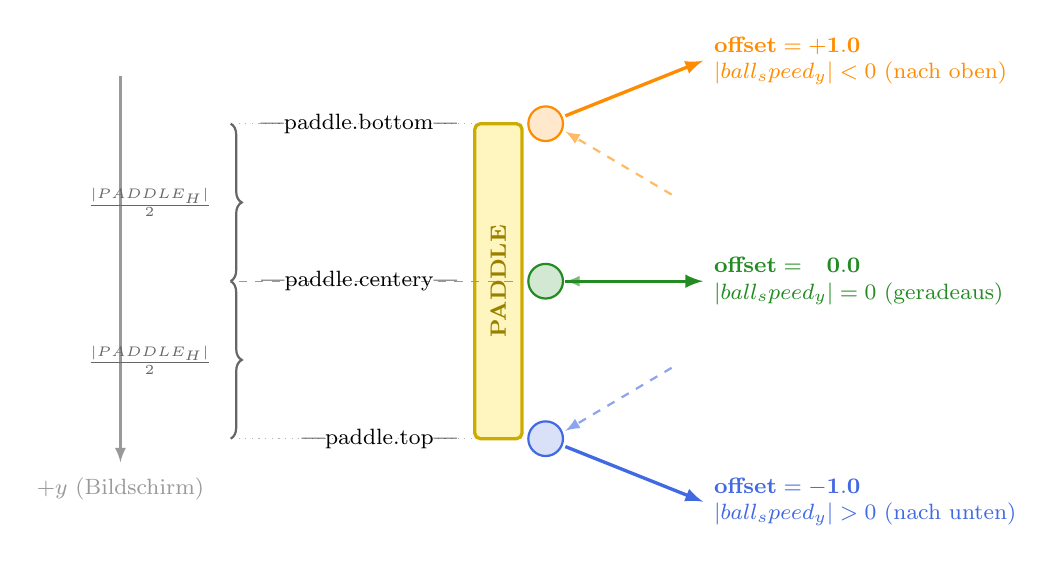
\begin{tikzpicture}[>=latex, font=\small]
                  % y-Achse (Pygame: nach unten positiv)
                  \draw[->, thick, gray!80] (-4.8, 2.6) -- (-4.8, -2.3)node[below=2pt] {\footnotesize $+y$ (Bildschirm)};
                  
                  % Paddle
                  \draw[fill=Gold!25, draw=Gold!80!black, very thick, rounded corners=2pt] (-0.3, -2.0) rectangle (0.3, 2.0);
                  \node[rotate=90, font=\footnotesize\bfseries, text=Gold!60!black] at (0, 0) {PADDLE};

                  % Mittellinie und Hilfslinien
                  \draw[dashed, black!40] (-3.3, 0) -- (0.3, 0);
                  \draw[dotted, black!30] (-3.3, -2.0) -- (-0.3, -2.0);
                  \draw[dotted, black!30] (-3.3, 2.0) -- (-0.3, 2.0);

                  % Beschriftungen links
                  \node[left, font=\footnotesize] at (-0.4, 0) {\lstinline|paddle.centery|};
                  \node[left, font=\footnotesize] at (-0.4, -2.0) {\lstinline|paddle.top|};
                  \node[left, font=\footnotesize] at (-0.4, 2.0) {\lstinline|paddle.bottom|};

                  % Bemassung PADDLE_H / 2
                  \draw[decorate, decoration={brace, amplitude=4pt, mirror}, thick, black!60] (-3.4, -2.0) -- (-3.4, 0)
                      node[midway, left=3pt, font=\scriptsize] {$\frac{\text{\lstinline|PADDLE_H|}}{2}$};
                  \draw[decorate, decoration={brace, amplitude=4pt, mirror}, thick, black!60] (-3.4, 0) -- (-3.4, 2.0)
                      node[midway, left=3pt, font=\scriptsize] {$\frac{\text{\lstinline|PADDLE_H|}}{2}$};

                  % Fall 1: Oben (-1.0) - RoyalBlue
                  \filldraw[fill=RoyalBlue!20, draw=RoyalBlue, thick] (0.6, -2.0) circle (0.22);
                  \draw[->, thick, dashed, RoyalBlue!60] (2.2, -1.1) -- (0.85, -1.9);
                  \draw[->, very thick, RoyalBlue] (0.85, -2.1) -- (2.6, -2.8) node[right, align=left, font=\footnotesize] {%
                      $\mathbf{\text{offset} = -1.0}$\\
                      $\implies \text{\lstinline|ball_speed_y|} > 0$ (nach unten)};

                  % Fall 2: Mitte (0.0) - ForestGreen
                  \filldraw[fill=ForestGreen!20, draw=ForestGreen, thick] (0.6, 0) circle (0.22);
                  \draw[->, thick, dashed, ForestGreen!60] (2.2, 0) -- (0.85, 0);
                  \draw[->, very thick, ForestGreen] (0.85, 0) -- (2.6, 0) node[right, align=left, font=\footnotesize] {%
                      $\mathbf{\text{offset} = \phantom{-}0.0}$\\
                      $\implies \text{\lstinline|ball_speed_y|} = 0$ (geradeaus)};

                  % Fall 3: Unten (+1.0) - DarkOrange
                  \filldraw[fill=DarkOrange!20, draw=DarkOrange, thick] (0.6, 2.0) circle (0.22);
                  \draw[->, thick, dashed, DarkOrange!60] (2.2, 1.1) -- (0.85, 1.9);
                  \draw[->, very thick, DarkOrange] (0.85, 2.1) -- (2.6, 2.8) node[right, align=left, font=\footnotesize] {%
                      $\mathbf{\text{offset} = +1.0}$\\
                      $\implies \text{\lstinline|ball_speed_y|} < 0$ (nach oben)};
              \end{tikzpicture}
              \end{center}

        \item \textbf{Ball nach Punkt neu zentrieren (als Funktion):}
              \begin{lstlisting}
def reset_ball(direction):  # direction: -1 nach links, +1 nach rechts
    global ball, ball_speed_x, ball_speed_y # Zugriff auf globale Variablen
    ball.center = (WIDTH // 2, HEIGHT // 2)
    ball_speed_x = direction * ball_speed
    ball_speed_y = random.choice((-1, 1)) * ball_speed
\end{lstlisting}

        \item \textbf{Nützliche Rect-Eigenschaften:} \lstinline|left, right, top, bottom, center, centery| helfen bei Ausrichtung und Kollisionen.
    \end{itemize}
\end{myattention}

\begin{mychallenge}[Pong-Bonus]
    Fügen Sie dem Pong-Spiel folgende Features hinzu:
    \begin{itemize}
        \item Soundeffekte bei Paddle-Kollision und Punktgewinn
        \item Startbildschirm mit Anweisungen
        \item Game-Over-Bildschirm nach einer bestimmten Punktzahl (z.\,B. 10 Punkte)
        \item Paddle-Geschwindigkeit erhöhen, wenn der Ball getroffen wird
        \item Hintergrundmusik während des Spiels
    \end{itemize}
\end{mychallenge}

\begin{myexercise}[Videoaufnahme des Spiels]
    Nehmen Sie ein kurzes Video (ca. 1-2 Minuten) auf, das das Gameplay Ihres Spiels zeigt. Laden Sie das Video auf eine Plattform (z.\,B. YouTube, Vimeo) hoch und fügen Sie den Link auf Moodle ein. Für die Bildschirmaufnahme können Sie folgende Tools verwenden:

    \begin{itemize}
        \item \textbf{Windows:} Verwenden Sie die Bildschirmaufnahme-Funktion von PowerPoint (unter \enquote{Einfügen} $\rightarrow$ \enquote{Bildschirmaufnahme}) oder die Xbox Game Bar (\keys{\faWindows + G}), beenden Sie die Aufnahme mit \keys{\cmd + \faWindows + R}
        \item \textbf{macOS:} Verwenden Sie die integrierte Bildschirmaufnahme (\keys{\shift + \cmd + 5}), beenden Sie die Aufnahme mit \keys{\cmd + \ctrl + Esc}
    \end{itemize}
\end{myexercise}

\subsection{Objektorientierte Spielobjekte mit Pygame-Sprites}
In komplexeren Spielen möchten wir häufig viele gleichartige Spielobjekte gleichzeitig verwalten -- beispielsweise Dutzende Münzen, Sterne, Hindernisse oder Laser-Schüsse. Bisher mussten wir Positionen, Bewegungen und Kollisionen für jedes Objekt einzeln mit separaten Variablen, Schleifen und Listen steuern.

Pygame stellt dafür mit \lstinline|pg.sprite.Sprite| und \lstinline|pg.sprite.Group| ein elegantes, objektorientiertes System bereit, das direkt an das Klassen-Konzept aus \cref{ch:K07_Klassen} anknüpft:
\begin{itemize}
    \item \textbf{Sprite (\lstinline|pg.sprite.Sprite|):} Eine Klasse für ein einzelnes sichtbares Spielelement. Jedes Sprite besitzt zwingend zwei Attribute:
    \begin{itemize}
        \item \lstinline|self.image|: Die Bildfläche (\lstinline|pg.Surface|) des Objekts.
        \item \lstinline|self.rect|: Das \lstinline|pg.Rect|-Objekt, welches Position und Hitbox definiert.
    \end{itemize}
    Zusätzlich wird meist eine Methode \lstinline|update(self)| implementiert, um Position und Verhalten pro Frame zu aktualisieren.
    \item \textbf{Sprite-Gruppe (\lstinline|pg.sprite.Group|):} Verwaltet mehrere Sprites gesammelt.
    \begin{itemize}
        \item \lstinline|gruppe.update()| ruft automatisch die \lstinline|update()|-Methode aller enthaltenen Sprites auf.
        \item \lstinline|gruppe.draw(screen)| zeichnet alle Sprites der Gruppe mit einem einzigen Befehl an deren jeweiliger \lstinline|rect|-Position.
    \end{itemize}
    \item \textbf{Effiziente Kollisionserkennung:} Funktionen wie \lstinline|pg.sprite.spritecollide(spieler, gruppe, dokill)| prüfen Kollisionen zwischen einem einzelnen Sprite und einer ganzen Gruppe in einer einzigen Code-Zeile. Ist \lstinline|dokill=True|, werden alle kollidierenden Sprites sofort automatisch aus der Gruppe gelöscht.
\end{itemize}

\begin{myexample}[Sprites und Sprite-Gruppen]
Folgender Code zeigt das Einsammeln mehrerer Münzen-Sprites mit automatischer Kollisionserkennung (\lstinline|spritecollide|). Kopieren Sie den Code in eine Datei \texttt{game\_sprites.py} und führen Sie ihn aus:
\lstinputlisting[language=Python]{Grundlagen_Info/00_Programmieren/Skript/Code/K08_Game/game_sprites.py}
\end{myexample}

\begin{myexercise}[Sammelobjekte mit Sprites verwalten]\label{myexercise:Sprites}
    Bauen Sie ein eigenes Sammelspiel oder erweitern Sie Ihr bestehendes Spiel mit Pygame-Sprites:
    \begin{enumerate}
        \item Erstellen Sie eine eigene Sprite-Klasse \lstinline|Muenze(pg.sprite.Sprite)| (oder \lstinline|Stern| / \lstinline|Hindernis|). Definieren Sie im Konstruktor \lstinline|__init__()| die Attribute \lstinline|self.image| (z.\,B. ein gelber Kreis oder ein geladenes Bild) und \lstinline|self.rect| an einer zufälligen Position im Fenster.
        \item Erstellen Sie eine Sprite-Gruppe \lstinline|muenzen_gruppe = pg.sprite.Group()| und fügen Sie in einer Schleife 15 bis 20 Münzen mit \lstinline|muenzen_gruppe.add(...)| hinzu.
        \item Erstellen Sie eine Spieler-Klasse \lstinline|Spieler(pg.sprite.Sprite)|, deren \lstinline|update()|-Methode die Tastatureingaben (\lstinline|pg.key.get_pressed()|) verarbeitet.
        \item Aktualisieren Sie in der Game-Schleife alle Sprites mit \lstinline|update()|, prüfen Sie das Einsammeln mit \lstinline|pg.sprite.spritecollide(spieler, muenzen_gruppe, True)| und zeichnen Sie alle Elemente mit \lstinline|draw(screen)|.
    \end{enumerate}
    \begin{myanswer}
        Diese Musterlösung finden Sie in \cref{sec:K09_sol}.
    \end{myanswer}
\end{myexercise}



\section{Dateiverarbeitung: Speicher- \& Highscore-Systeme (File I/O)}
Damit ein Game Spielstände, Einstellungen oder Highscores auch nach dem Beenden des Programms behält, müssen Daten dauerhaft auf dem Datenträger gespeichert werden. In Python erfolgt der Dateizugriff am sichersten mit dem \lstinline|with open(...)|-Konstrukt, welches sicherstellt, dass die Datei nach dem Bearbeiten automatisch geschlossen wird.

\subsection{Einfache Textdateien (.txt)}
Mit dem Modus \lstinline|"r"| (Read) werden Daten gelesen, mit \lstinline|"w"| (Write) überschrieben und mit \lstinline|"a"| (Append) angefügt.

\begin{mydefinition}[Dateien lesen und schreiben]
\begin{lstlisting}
# Highscore in Datei schreiben
highscore = 250
with open("highscore.txt", "w", encoding="utf-8") as file:
    file.write(str(highscore))

# Highscore aus Datei lesen
with open("highscore.txt", "r", encoding="utf-8") as file:
    content = file.read().strip()
    highscore = int(content)
\end{lstlisting}
\end{mydefinition}

\begin{myexercise}[Highscore-Speicher in Pygame]\label{myexercise:HighscoreTxt}
Schreiben Sie zwei Hilfsfunktionen \lstinline|load_highscore()| und \lstinline|save_highscore(score)| für Ihr Game:
\begin{enumerate}
    \item \lstinline|load_highscore()| prüft mit \lstinline|os.path.exists("highscore.txt")|, ob die Datei existiert. Falls ja, liest sie die Zahl aus und gibt sie als \lstinline|int| zurück. Falls nicht (oder bei einem Fehler), gibt sie \lstinline|0| zurück.
    \item \lstinline|save_highscore(score)| schreibt den neuen Punktestand in die Datei \texttt{highscore.txt}.
\end{enumerate}
\end{myexercise}

\subsection{Strukturierte Tabellen mit CSV (.csv)}
Möchte man eine Rangliste (Leaderboard) mit mehreren Spielernamen und Punkteständen speichern, eignet sich das CSV-Format (Comma-Separated Values). Python bietet dafür das eingebaute Modul \lstinline|csv|.

\begin{mydefinition}[CSV-Dateien lesen und schreiben]
\begin{lstlisting}
import csv

# Leaderboard speichern
scores = [["Alice", 240], ["Bob", 180], ["Clara", 310]]
with open("highscores.csv", "w", newline="", encoding="utf-8") as file:
    writer = csv.writer(file)
    writer.writerow(["Player", "Score"])  # Header
    writer.writerows(scores)

# Leaderboard laden
with open("highscores.csv", "r", encoding="utf-8") as file:
    reader = csv.reader(file)
    next(reader, None)  # Header-Zeile überspringen
    for row in reader:
        player_name = row[0]
        player_score = int(row[1])
\end{lstlisting}
\end{mydefinition}

\begin{myexercise}[Leaderboard-Tabelle mit CSV]\label{myexercise:HighscoreCsv}
Implementieren Sie eine Funktion \lstinline|load_leaderboard()|, welche die CSV-Datei \texttt{highscores.csv} einliest, die Einträge nach Punktestand absteigend sortiert und die Top-3-Spieler auf der Konsole oder im Pygame-Fenster ausgibt.
\end{myexercise}

\section{Game-Auftrag}

\subsection{Thema}
Im Folgenden wählen Sie in Zweier-Gruppen (bei ungrader Anzahl Personen eine Dreiergruppe möglich) ein Game-Thema aus und entwickeln ein 2D-Game mit \texttt{pygame-ce}. Mögliche Themen sind:
\begin{itemize}
    \item \textbf{Sammelspiel:} Bewegen Sie eine Spielfigur (z.\,B. Auto, Raumschiff) und sammeln Sie Items ein (z.\,B. Treibstoff, Sterne). Jedes eingesammelte Item gibt Punkte.
    \item \textbf{Endlos-Runner:} Steuern Sie eine Spielfigur (z.\,B. Läufer, Auto) und weichen Sie Hindernissen aus (z.\,B. Mauern, andere Autos). Jedes überstandene Hindernis gibt Punkte.
    \item \textbf{Fangspiel:} Steuern Sie eine Spielfigur (z.\,B. Katze, Netz) und fangen Sie herumspringende Objekte (z.\,B. Mäuse, Schmetterlinge). Jedes gefangene Objekt gibt Punkte.
    \item \textbf{Shooter (z.B. Space Invaders):} Steuern Sie ein Raumschiff und schiessen Sie auf herannahende Gegner. Jeder abgeschossene Gegner gibt Punkte.
\end{itemize}

Weitere Themen können in Absprache mit der Lehrperson gewählt werden. Wichtig ist, dass das Spiel die geforderten Python-Konzepte sinnvoll einsetzt (siehe Anforderungen) und die Komplexität angemessen ist (nicht zu einfach, aber auch nicht zu komplex). Das Spiel sollte mehr als nur 10 Sekunden lang Spass machen und nicht zu einfach zu spielen sein. Es sollte eine Herausforderung darstellen, die Spieler motiviert, immer wieder zu spielen und ihre Punktzahl zu verbessern.

\subsection{Anforderungen}

Ihr Projekt sollte folgende, essentielle Python-Konzepte sinnvoll einsetzen
\begin{todolist}
    \item Verwendung von \texttt{pygame-ce} für Fenster, Game-Schleife, Ereignisse, Zeichnen, Kollisionen und Medien (Bilder, Sound), Steuerung mit Tastatur und/oder Maus
    \item Verwendung physikalischer Formeln für Bewegungen (z.\,B. Geschwindigkeit, Beschleunigung, Schwerkraft)
    \item Verwendung von \textbf{Variablen} zur Speicherung von Spielzuständen (z.\,B. Spielerposition, Punktestand, verbleibende Zeit)
    \item Verwendung von \textbf{Funktionen} zur Strukturierung des Codes (z.\,B. \lstinline|draw_player()|, \lstinline|update_game()|, \lstinline|handle_input()|), mit sowie ohne \lstinline|return|-Wert
    \item Verwendung von \textbf{logischen Ausdrücken} und \textbf{Schleifen} zur Steuerung des Spielablaufs (z.\,B. Kollisionserkennung, Punkte zählen, Spielzeit)
    \item Verwendung von \textbf{Datenstrukturen} (Listen, Dictionaries) zur Verwaltung von mehreren Spielobjekten (z.\,B. Liste von Items, Liste von Hindernissen)
    \item Verwendung von \textbf{Klassen} zur Modellierung von Spielobjekten (z.\,B. \lstinline|class Player|, \lstinline|class Item|, \lstinline|class Obstacle|)
    \item Verwendung mehrerer Python-Unterdateien zur besseren Strukturierung des Codes (z.\,B. \lstinline|game.py|, \lstinline|player.py|, \lstinline|item.py|)
\end{todolist}

Ihr Game muss \textbf{Kommentare} enthalten, die den Code erklären und die Struktur des Programms verdeutlichen. Verwenden Sie sowohl einzeilige Kommentare (mit \lstinline|#|) als auch mehrzeilige Kommentare (mit \texttt{"""..."""}) für Funktionen und Klassen. \textbf{Schauen Sie sich die detaillierten Bewertungskriterien auf Moodle an, um sicherzustellen, dass Ihr Code den Anforderungen entspricht.}

\subsection{Bonus}

\begin{todolist}
    \item Python-spezifisch:
    \begin{todolist}
        \item Verwendung von \texttt{try/except} zur Behandlung von Fehlern (z.\,B. Laden von Medien, Division durch Null)
        \item Verwendung von \texttt{with}-Anweisung zum sicheren Öffnen und Schliessen von Dateien (z.\,B. Highscore speichern)
        \item Wenn Sie ein Punktesystem mit Highscore (gespeichert in einer Datei) implementieren.
    \end{todolist}
    \item Game-spezifisch:
    \begin{todolist}
        % \item Wenn Sie ein Startmenü und/oder ein Game-Over-Bildschirm implementieren.
        % \item Wenn Sie Animationen (z.\,B. bewegte Spielfigur, animierte Hindernisse) einbauen.
        % \item Wenn Sie verschiedene Level oder Schwierigkeitsgrade (z.\,B. schnellere Hindernisse, mehr Items) implementieren.
        \item Wenn Sie viele Power-Ups (z.\,B. temporäre Unverwundbarkeit, Doppelte Punkte) einbauen.
        \item Wenn Sie viele eigens erstellte Hintergrundmusik und/oder Soundeffekte (z.\,B. bei Kollision, Item-Sammlung) einbauen.
        \item Wenn Sie das Spiel mit einem Gamepad/Controller steuern können.
        \item Wenn Sie einen Online-Multiplayer-Modus (z.\,B. über LAN) implementieren.
    \end{todolist}
    \item Weitere Ideen für Bonus:
    \begin{todolist}
        \item Wenn Sie das Spiel mit einem Level-Editor (zum Erstellen eigener Level) erweitern können.
        \item Wenn Sie das Spiel mit einem Story-Modus (mit Handlung und Charakteren) erweitern können.
        \item Wenn Sie das Spiel mit einem besonders raffinierten Achievements-System (Erfolge) erweitern können.
        \item Wenn Sie das Spiel mit einem Debug-Modus (zum Testen und Entwickeln) erweitern können.
    \end{todolist}
\end{todolist}

\section{Bewertung}
\subsection{Projektbewertung}
Die Bewertung Ihres Projekts erfolgt anhand der auf Moodle aufgelisteten Kriterien.

\subsection{Gruppen-Besprechung des Spiels}

Im Anschluss an Ihre Abgabe findet eine Besprechung Ihres Spiels in Gruppen mit der Lehrperson statt (ca. 5 Minuten pro Person). Dabei werden Ihnen Fragen zu Ihrem Spiel gestellt, um Ihr Verständnis und Ihre Reflexion zu überprüfen. Die Besprechung resultiert in einer \textbf{individuellen} Verständnis-Punktzahl von bis zu 16 Punkten, welche mit Ihrer Endnote multipliziert wird:

Ihre Endnote wird wie folgt berechnet:
\[\text{Endnote} = \text{Projekt-Note} + \Delta_{\text{Verständnis}}\]

Wobei:
\begin{itemize}
    \item \textbf{Projekt-Note} die Note ist, die Sie basierend auf der Bewertung Ihres Projekts erhalten (0--100 Punkte, umgerechnet in Notenstufen)
    \item \textbf{Verständnis-Delta} ein Bonus oder Malus ist, abhängig von Ihrer Verständnis-Punktzahl (0--16 Punkte), wie folgt:
    \begin{itemize}
        \item 14 Punkte: $\Delta = 0$ (keine Veränderung)
        \item 15 Punkte: $\Delta = +0.1$
        \item 16 Punkte: $\Delta = +0.2$
        \item Unter 14 Punkte: lineare Verschlechterung, maximal $\Delta = -1$ Note
    \end{itemize}
\end{itemize}

\begin{myattention}[KI-Tools]
    Es wird von Ihnen erwartet, dass Sie sich aktiv an der Entwicklung des Spiels beteiligen und die geforderten Python-Konzepte verstehen und anwenden können. ChatGPT oder andere KI-Tools dürfen Sie verwenden, solange Sie Ihren gesamten Code verstehen und erklären können. Wie Sie im obigen Benotungsschema erkennen können, kann Ihre Note durch mangelndes Verständnis stark beeinträchtigt werden. Falls Sie ChatGPT oder andere KI-Tools verwenden, müssen Sie dies im Code klar dokumentieren (z.B. mit Kommentaren oder in einer Begleit-Dokumentation). Jede Zeile Code muss durch Sie erklärbar sein!
\end{myattention}


\iftoggle{exerciseonly}{}{%
	\clearpage

	\section{Längere Lösungen}\label{sec:K09_sol}

	\begin{myanswer}[myexercise:Sonnenuntergang]
		\leavevmode %
        \lstinputlisting[language=Python,caption=\texttt{game\_intro\_sunset.py},label=listing:Sonnenuntergang]{Grundlagen_Info/00_Programmieren/Skript/Code/K08_Game/game_intro_sunset.py}
	\end{myanswer}

    \begin{myanswer}[myexercise:Bewegungen]
		\leavevmode %
        \lstinputlisting[language=Python,caption=\texttt{game\_intro\_player\_rect.py},label=listing:Bewegungen]{Grundlagen_Info/00_Programmieren/Skript/Code/K08_Game/game_intro_player_rect.py}
	\end{myanswer}

    \begin{myanswer}[myexercise:Kollisionen]
        \leavevmode %
        \lstinputlisting[language=Python,caption=\texttt{game\_intro\_collision.py},label=listing:Kollisionen]{Grundlagen_Info/00_Programmieren/Skript/Code/K08_Game/game_intro_collision.py}
    \end{myanswer}

    \begin{myanswer}[myexercise:Highscore]
        \leavevmode %
        \lstinputlisting[language=Python,caption=\texttt{game\_intro\_highscore.py},label=listing:Highscore]{Grundlagen_Info/00_Programmieren/Skript/Code/K08_Game/game_intro_highscore.py}
    \end{myanswer}

    \begin{myanswer}[myexercise:Ereignisse]
        \leavevmode %
        \lstinputlisting[language=Python,caption=\texttt{game\_intro\_events.py},label=listing:Ereignisse]{Grundlagen_Info/00_Programmieren/Skript/Code/K08_Game/game_intro_events.py}
    \end{myanswer}

    \begin{myanswer}[myexercise:Medien]
        \leavevmode %
        \lstinputlisting[language=Python,caption=\texttt{game\_intro\_media.py},label=listing:Medien]{Grundlagen_Info/00_Programmieren/Skript/Code/K08_Game/game_intro_media.py}
    \end{myanswer}

    \begin{myanswer}[myexercise:Sprites]
        \leavevmode %
        \lstinputlisting[language=Python,caption=\texttt{game\_sprites.py},label=listing:Sprites]{Grundlagen_Info/00_Programmieren/Skript/Code/K08_Game/game_sprites.py}
    \end{myanswer}

    \begin{myanswer}[myexercise:HighscoreTxt]
        \leavevmode %
        \lstinputlisting[language=Python,caption=\texttt{game\_highscore\_txt.py},label=listing:HighscoreTxt]{Grundlagen_Info/00_Programmieren/Skript/Code/K08_Game/game_highscore_txt.py}
    \end{myanswer}

    \begin{myanswer}[myexercise:HighscoreCsv]
        \leavevmode %
        \lstinputlisting[language=Python,caption=\texttt{game\_highscore\_csv.py},label=listing:HighscoreCsv]{Grundlagen_Info/00_Programmieren/Skript/Code/K08_Game/game_highscore_csv.py}
    \end{myanswer}
}